\chapter{Implementação e Resultados}
\label{Capitulo: Resultados}

Consideraremos $N$ partículas em um subespaço $S$ de dimensão $d$ em $\mathbb{R}^n$ de forma que nosso espaço de fase $\Omega$ será de dimensão $Nd$. O campo externo é $V : S \mapsto \mathbb{R}$ e o núcleo de interação entre as partículas é função $\W : S \mapsto (-\infty, \infty]$. Reunindo os resultados do Capítulo \ref{Capitulo: Simulações} sob essas condições, temos o algoritmo, com base em Chafa\"{i} e Ferré \cite{Chafa2018}, completo. Dada uma condição inicial $(q_k, p_k)$,  vetores de posição e momento generalizados, para cada $k\geq0$, realizamos os seguintes passos
\begin{enumerate}
	\item Baseado na Equação \eqref{Equation: Mehler}, atualize $\tilde{p}_k$ com
	\begin{equation}
	\tilde{p}_k = \eta p_k + \sqrt{\frac{1-\eta^2}{\beta_N}} G_k, \ \eta = \ee^{-\gamma_N \alpha_N \Delta t};
	\label{Equation: Alg Mehler}
	\end{equation}
	\item Utilizando do esquema de Verlet \eqref{Equation: Verlet}, calcule os termos
	\begin{equation}
	\begin{cases}
		\tilde{p}_{k+\frac{1}{2}} = \tilde{p}_k - \nabla \Hf_N(q_k) \alpha_N \frac{\Delta t}{2}, \\
		\tilde{q}_{k+1} = q_k + \tilde{p}_{k + \frac{1}{2}} \alpha_N \Delta t, \\
		\tilde{p}_{k+1} = \tilde{p}_{k+\frac{1}{2}} - \nabla \Hf_N(\tilde{q}_{k+1}) \alpha_N \frac{\Delta t}{2};
		\label{Equation: Alg Verlet}
	\end{cases}
	\end{equation}
	\item Pela Definição \eqref{Equation: Pk}, tome
	\begin{equation}
	P_k = 1 \wedge \exp{ -\beta_N \left(\Ee_N(\tilde{q}_{k+1}, \tilde{p}_{k+1}) - \Ee_N(q_{k}, \tilde{p}_{k}) \right)};
	\label{Equação: Alg Pk}
	\end{equation}
	\item Defina, a partir da Razão \eqref{Equation: Metropolis}, 
	\begin{equation}
	(q_{k+1}, p_{k+1}) = 
	\begin{cases}
		(\tilde{q}_{k+1}, \tilde{p}_{k+1}) \ \text{com probabilidade} \ P_k, \\
		(q_k, -\tilde{p}_{k}) \ \text{com probabilidade} \ 1-P_k; \\
	\end{cases}
	\label{Equation: Alg Metro}
	\end{equation}
\end{enumerate}

% -
% C3S1 - A implementação
% - 
\section{A implementação}

Tomaremos o subespaço $\Se = \R^d$ com $d = 1, 2$. Consideraremos um núcleo de interação $\W = g$ coulombiano em $n = 2$. Por isso, retomamos medida da forma \ref{Equação: Medida Gas de Coulomb} usual de gases de coulomb. A esquemática da implementação se encontra na Figura \ref{Figura: Implementação}. Podemos entender melhor a relação entre as sub-rotinas e funções em referência à Tabela \ref{Table: Funcoes e Subrotinas}.

\begin{figure}[ht]
	\centering
	\begin{tikzpicture}[font=\tiny,thick]
		
		% Start block
		\node[subrotina] (INIT) {INIT};
		
		% -------------------------------------------------------------------		
		
		\node[subrotina,
		left=0.2cm of INIT] (LabelSubrotina) {Subrotinas};
		
		\node[funcao,
		below=0.1cm of LabelSubrotina] (LabelFunção) {Funções};
		
		% -------------------------------------------------------------------		
		
		\node[funcao,
		below=0.1cm of INIT, xshift=2cm] (Hold) {H};
		
		\node[funcao,
		right=0.5cm of Hold, yshift=0.3cm] (Wold) {W};
		
		\node[funcao,
		right=0.5cm of Hold, yshift=-0.3cm] (Vold) {V};
		
		
		\node[loop,
		below=1cm of INIT,
		minimum width=6cm,
		xshift=2cm,
		] (LOOP) {
			\begin{tikzpicture}
				
				\node[subrotina,
				] (L2) {L2-OrnsUhlen};
				
				\node[funcao,
				below=0.5cm of L2
				] (Gauss) {Gauss};
				
				\node[subrotina,
				right=2cm of L2] (L1) {L1-Verlet};
				
				\node[subrotina,
				below=0.5cm of L1] (GradH) {GradH};
				
				\node[subrotina,
				below=0.5cm of GradH, xshift=1cm] (GradW) {GradW};
				
				\node[subrotina,
				below=0.5cm of GradH, xshift=-1cm] (GradV) {GradV};
								
				\node[subrotina,
				below=3cm of L2, xshift=-0.5cm] (Metro) {Metropolis};
				
				\node[funcao,
				below=0.3cm of Metro
				] (Problog) {ProbLog};
				
				\node[funcao,
				right=1cm of Problog] (H) {H};
				
				\node[funcao,
				right=0.5cm of H, yshift=0.3cm] (W) {W};
				
				\node[funcao,
				right=0.5cm of H, yshift=-0.3cm] (V) {V};
				
				\node[random,
				above=0.5cm of Metro, xshift=-1.3cm] (aceito) {$q_k = \tilde{q}_{k_1}$ \\ $p_k = \tilde{p}_{k_1}$};
				
				\node[random,
				above=0.5cm of Metro, xshift=1.3cm] (negado) {$q_k = q_k$ \\ $p_k = -p_k$};
				
				
				% ---------------------------------------------------------------------
				
				\path [fluxo] (L2) -- (L1);
				\path [fluxo]  (L2) ++(-3cm, 0cm) -- (L2);
				\path [chamada] (L2) -- (Gauss);
				\path [chamada] (L1) -- (GradH);
				\path [chamada] (GradH) -- (GradV);
				\path [chamada] (GradH) -- (GradW);
				\path [fluxo]  (L1) --++(2cm, 0cm) |- (Metro);
				\path [chamada] (Metro) -- (Problog);
				\path [chamada] (Problog) -- (H);
				\path [chamada] (H) -- (W);
				\path [chamada] (H) -- (V);
				\path [meiofluxo] (Metro) -- (aceito);
				\path [meiofluxo] (Metro) -- (negado);
				\path [meiofluxo] (negado) -- ++(0cm, 0.8cm) -- ++(-2.6cm, 0cm);
				\path [meiofluxo] (aceito) -- ++(0cm, 1.5cm);
				\path [fluxo] (aceito)++(0cm, 1.45cm) -- ++(0cm, 0.8cm);
				
			\end{tikzpicture}
		};
	
		\node[random,
		left=0.3cm of LOOP,
		yshift=2cm,
		rotate=90
		] (do) {DO k = 1, nsteps};
		
		\path [fluxo] (INIT) -- ++(0cm, -1.3cm);
		\path [chamada] (INIT) ++(0cm, -0.7cm) -- (Hold);
		\path [chamada] (Hold) -- (Vold);
		\path [chamada] (Hold) -- (Wold);
		
	\end{tikzpicture}
\caption{Implementação do algoritmo \textit{Langevin Monte Carlo} (LMC). Setas sólidas indicam o fluxo do programa. Setas tracejadas indicam chamadas de funções dentro do bloco. A descrição das funções se encontra na Tabela \ref{Table: Funcoes e Subrotinas}.}
\label{Figura: Implementação}
\end{figure}

\begin{table}[ht]
	\centering
	\begin{tabular}{ |p{2.6cm}||p{12cm}|  }
		\hline
		Nome & Descrição \\ 
		\hline
		\hline
		Init   		  	 & 
		Modifica ${p}_{k}$ vetor $[N\times m]$, global, uniforme no cubo em $R^d$ e ${q}_{k}, G_H$, vetores $[N\times m]$, globais, nulos. \\
		\hline
		L1-OrnsUhlen 	 & 
		Modifica $\tilde{p}_k$, vetor $[N\times m]$, global, por $\Gl_U$ segundo \ref{Equation: Alg Mehler}. \\
		\hline
		L2-Verlet  	 	 & 
		Modifica $\tilde{p}_{k_1},\tilde{q}_{k_1}$ vetores $[N\times m]$, globais, por $\Gl_{\Hf}$ segundo \ref{Equation: Alg Verlet}.	\\
		\hline
		GradH         	 & 
		Modifica $G_H$, vetor $[N\times m$], global, gradiente do Hamiltoniano.					\\
		\hline
		GradW        	 &
		Modifica $G_{W_i}$, escalar, global, gradiente de $W$ núcleo de interação.	\\
		\hline
		GradV  	      	 &
		Modifica $G_{V_i}$, escalar, global, gradiente de $\V$ potencial.		                    \\
		\hline
		ProbLog       		 &
		Retorna $P_K$, escalar, local, probabilidade de aceite de \ref{Equação: Alg Pk}. \\
		\hline
		H              	 &
		Retorna $H$, escalar, local, hamiltoniano em $k$.	 							\\
		\hline
		V  	      			 &
		Retorna $V_i$, escalar, local, potencial de $q_i$.								\\
		\hline
		W         	  		 & 
		Retorna $W_{i,j}$, escalar, local, interação entre $q_i,q_j$ 							\\
		\hline
		Metropolis     	 & 
		Modifica ${p}_{k},{q}_{k}$, vetores $[N\times m]$, globais por \ref{Equation: Alg Metro}.								\\
		\hline
	\end{tabular}
	\caption{ Descrição das funções e subrotinas utilizadas na implementação do programa.}
	\label{Table: Funcoes e Subrotinas}
\end{table}

 Alguns detalhes são importantes de notar. O gerador de variáveis aleatórias gaussianas, necessário em \ref{Equation: Alg Mehler} foi implementado utilizando do algoritmo de \textit{Box-Muller}. Além disso, o ajuste de variáveis é notoriamente um dos aspectos complicados do algoritmo implementado. Precisamos de uma holística par ajustar $\Delta t, \alpha_N \ \text{e} \ \gamma_N$. No escopo deste programa, $\Delta t$ e $\alpha_N$ desempenham o mesmo papel e, por isso, toma-se $\alpha_N = 1$ e varia-se $\Delta t$. Seguindo a recomendação de \cite[Capítulo~5]{handbookmontecarlo}, tomaremos $\Delta t = \Delta\tilde{t} + X$, onde $X$ é variável aleatória de média $0$ e variância $\sigma^2$ pequena. Essa escolha ajuda a acelerar a convergência e melhor garante ergoticidade. Lembra-se ainda que $\Delta \tilde{t}$ é ideal na ordem de $N^{-\frac{1}{4}}$, isto é, é pequeno o suficiente para manter a razão de aceite do passo de Metropolis alta e grande o suficiente para não desacelerar a convergência do algoritmo. Já $\gamma_N$ definirá o quanto substituiremos o momento anterior das partículas será relevante em relação ao movimento browniano. Aqui, sabemos que tornar $\eta$ próximo demais de $0$, ou de $1$ para todos efeitos, desacelera intensamente a convergência. Faremos, em geral, com que $\gamma_N \alpha_N \Delta t \approx 0.5$.
 
 %Para além dos ajustes, cada simulação é identificada pelo Hamiltoniano, ou seja, pelo potencial $V$ e pelas dimensões $d, n$, respectivamente do espaço que as partículas estão restritas e do que elas existem.




% -
% C3S2 - Validação em distribuições conhecidas
% - 
\section{Resultados e Discussão}

Simular Gases de Coulomb é especialmente interessante quando não há modelos de matrizes conhecidos, disponíveis ou simples para o $\Hf$ tomado. Podemos, com a simulação de tais gases, calcular a média da função densidade das partículas, ou autovalores, sem ter que diretamente lidar com as matrizes correspondentes. Alternativamente, quando há modelos disponíveis na teoria de RMT, as matrizes poderiam ser diretamente amostradas e a função dos autovalores calculada da diagonalização das mesmas. Tratemos de um caso onde ambas as abordagens são possíveis.

A família de ensembles gaussianos são modelos que mostramos ser bem representados como matrizes na Seção \ref{Section: Ensembles Gaussianos}. Retorne os resultados da Seção \ref{Section: Potencias}. Tomar a medida dos ensembles gaussianos é o equivalente, na simulação de gases descrita, a tomar 
\begin{equation}
d = 1; \ \  n = 2; \ \ \V(x)=\frac{|x|^2}{2}; \ \ W(x) = g(x) = \log{|x|}; \ \ \beta_N = \beta N^2; \ \ \beta = 1,2,4.
\label{Equation: Parametros Gaussian}
\end{equation}
O resultado da simulação para a Configuração \eqref{Equation: Parametros Gaussian} é apresentado na Figura \ref{Figura: Gaussian} para os três modelos ($\beta = 1,2,4$). Na coluna da esquerda, contrasta-se os resultados para $N=10$ da densidade gerada por ambas a simulação de gases e a amostragem direta de matrizes do ensemble. Na coluna central, representa-se a comparação da medida da simulação com o Semi-Círculo de Wigner, configuração de equilíbrio para os três modelos quando $N$ é grande o suficiente. Note que os valores foram escalados por $\sqrt{2 \beta}$ para apresentarem mesmo suporte. Finalmente, na coluna da direita apresentamos a distribuição do maior autovalor $\lambda_{max}$. Um resultado importante enuncia que existem $z_{N}^{(\beta)}$ e $s_N^{(\beta)}$ tais que $$\lim_{N \to \infty} \mathbb{P}_{\beta,N,V} \left( \frac{\lambda_{max} - z_{N}^{(\beta)}}{s_N^{(\beta)}} \leq x \right) = F_{\beta}(x),$$ onde $F_{\beta}(x)$ é a densidade acumulada de Tracy-Widow. \cite{Tracy} 

Observa-se que os dois modelos à esquerda, amostragem direta e simulação de gases, concordam bem na estimativa da medida para o $N$ usado. No centro, é possível notar que a medida de equilíbrio esperada, o Semi-Círculo de Wigner, é aproximada rapidamente pelo aumento de partículas no sistema. A distribuição do autovalor máximo é mais delicada; contudo, ainda que com $N$ finito, podemos ver boa correspondência com o resultado esperado pela Tracy-Widow, piorando com a diminuição da temperatura.
\begin{figure}[ht!]
	\centering
	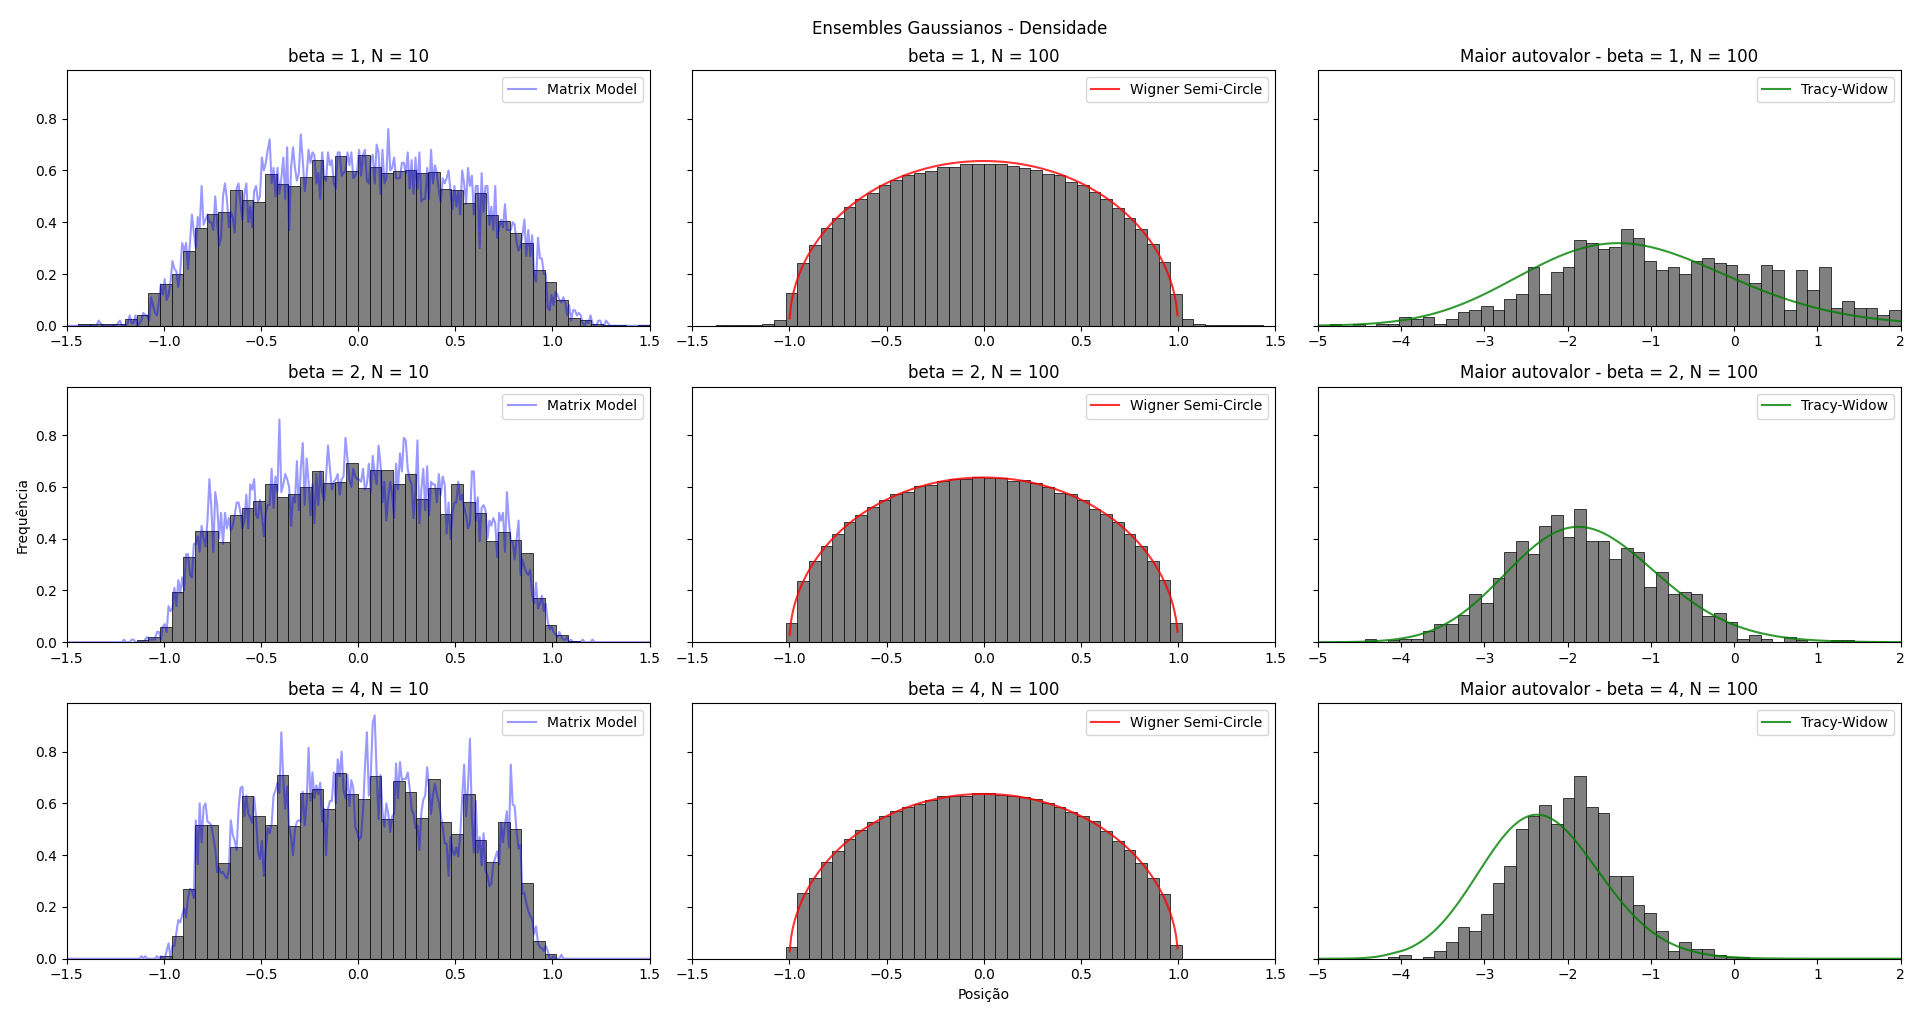
\includegraphics[width=\textwidth]{Assets/validationGaussianTracy.png}
	\caption{Densidade para ensembles gaussianos, \eqref{Equation: Parametros Gaussian}. Tomou-se $\Delta \tilde{t} = 0.1$ e $nsteps = 5\cdot10^6$ passos, registrando a cada $100$ iterações a partir de $nsteps/5$. À esquerda da figura, em azul, a densidade da amostragem de $4\cdot10^3$ matrizes do ensemble. No centro, o Semi-Círculo de Wigner, medida de equilíbrio. Na direita, apresenta-se a densidade de $\lambda_{max}$ normalizado e sua medida esperada.}
	\label{Figura: Gaussian}
\end{figure}

Podemos retomar também as descrições dos potenciais mônico, na Equação \eqref{Equação: Mônico}, e os dois regimes do potencial quártico, Caso \eqref{Equação: Quartico +} e Caso \eqref{Equação: Quartico -}. Respectivamente, estes modelos equivalem a tomar na simulação os parâmetros
\begin{equation}
	d = 1; \ \  n = 2; \ \ \V(x)= t |x|^{2m}; \ \ W(x) = g(x) = \log{|x|}; \ \ \beta_N = \beta N^2; \ \ \beta = 2.
	\label{Equation: Parametros Monico}
\end{equation}
\begin{equation}
	d = 1; \ \  n = 2; \ \ \V(x)=\frac{|x|^4}{4} + t \frac{|x|^2}{2}; \ \ W(x) = g(x) = \log{|x|}; \ \ \beta_N = \beta N^2; \ \ \beta = 2.
	\label{Equation: Parametros Quartico}
\end{equation}
O caso mônico se reduz ao gaussiano se $m=1$. Os resultados para ambos os potenciais estão explicitados na Figura \ref{Figura: Quartic Monic} para alguns parâmetros interessantes de $t$ e $m$.
\begin{figure}[ht!]
	\centering
	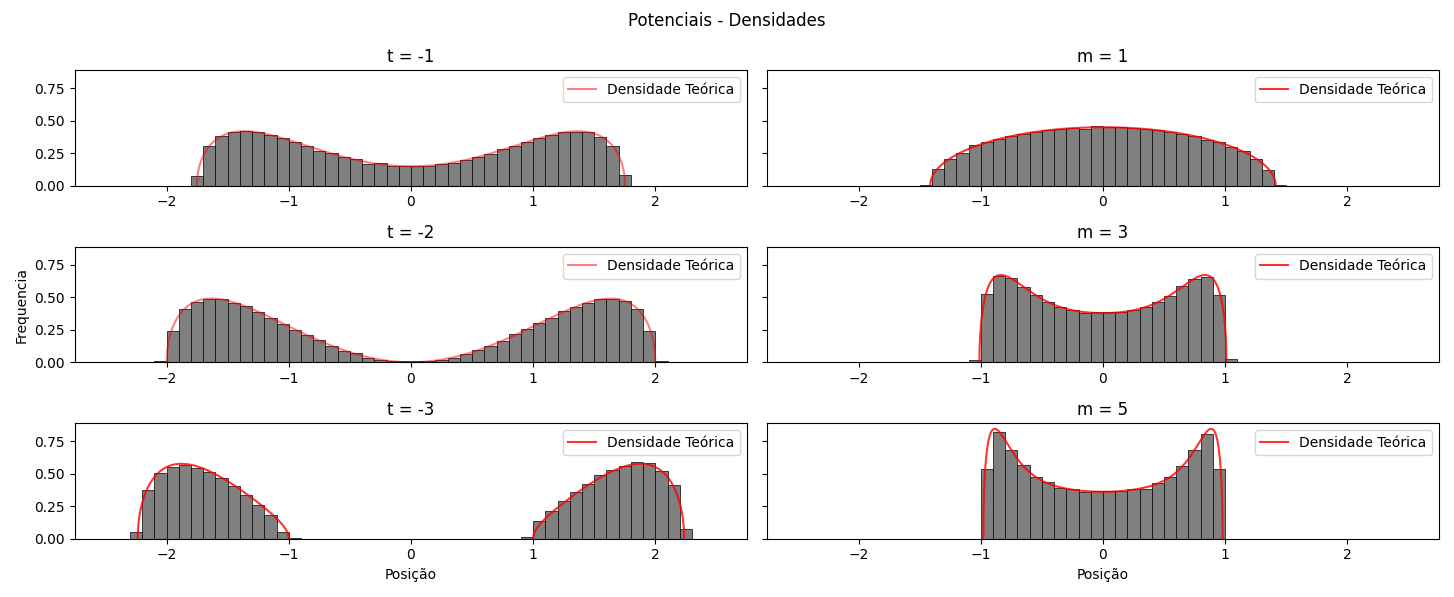
\includegraphics[width=\textwidth]{Assets/validationQuarticMonic-alt.png}
	\caption{Potencial Quártico \eqref{Equation: Parametros Quartico} e Mônico \eqref{Equation: Parametros Monico}, respectivamente à esquerda e direita. Tomou-se $\Delta \tilde{t} = 0.1$, $N=100$, e $nsteps = 5\cdot10^6$ passos. Registra-se a cada $1000$ iterações a partir de $nsteps/5$. No Quártico, simula-se $t=-1,-2,-3$. No Mônico fixa-se $t=1$ e simula-se $m=1,3,5$.}
	\label{Figura: Quartic Monic}
\end{figure}

Novamente as medidas experimentais parecem convergir para a medida teórica enunciada em todas as configurações testadas. Contudo, isso é discutido, com exceção do Mônico, por Chafa\"{i} e Ferré \cite{Chafa2018}. Em luz da situação recentemente explorada por Balogh \textit{et al.} \cite{balogh2016orthogonal} consideremos a Configuração \eqref{Equation: Complex} complexa. Para esta, representamos as medidas simuladas para alguns valores de interesse de $t, a$ na Figura \ref{Figura: Complex},
\begin{equation}
	d = 2; \  n = 2; \  \V(z)=|z|^{2a} - \Re{t z^a};  \ W(x) = g(x) = \log{|x|};  \ \beta_N = \beta N^2;  \ \beta = 2.
	\label{Equation: Complex}
\end{equation}

\begin{figure}[ht]
	\centering
	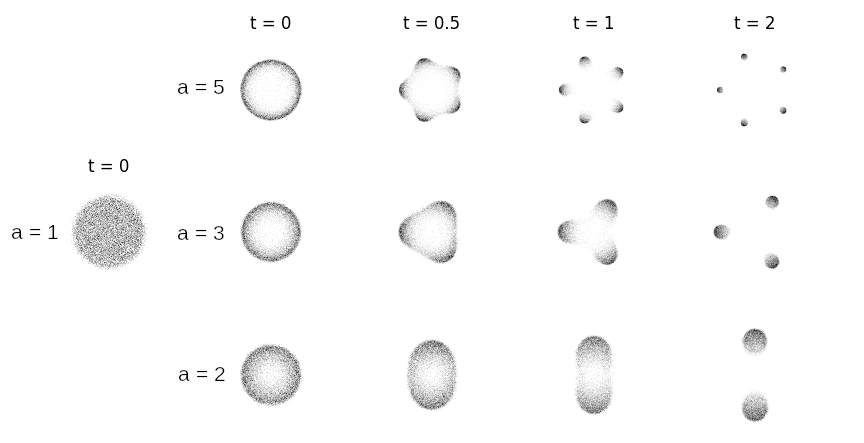
\includegraphics[width=\textwidth]{Assets/complexPotential.png}
	\caption{Medidas referentes à configuração \eqref{Equation: Complex}. Tomou-se $\Delta \tilde{t} = 0.5$ e $nsteps = 2\cdot10^6$ passos, registrando a cada $500$ iterações a partir de $nsteps/5$.}
	\label{Figura: Complex}
\end{figure}

É previsto para esse modelo uma transição de regime - uma separação da medida de equilíbrio - para $t_c \approx \sqrt{\frac{1}{a}}$, o que pode ser observado na Figura \ref{Figura: Complex} com algum detalhe. Outros fatores que corroboram o bom comportamento do modelo são que a medida é uniforme no disco quando $(a,t) = (1,0)$ e se concentra no bordo quando incrementa-se $a$, fatos também previstos. \cite{balogh2016orthogonal} Esse exemplo demonstra que é possível, sem muito esforço, replicar a medida, e principalmente o suporte, para potenciais mais complexos estudados em publicações recentes no tema e pode ser estendido para outros estudos, como para o potencial discutido por Bleher e Silva \cite{Silva}. 

No Capítulo \ref{Capitulo: Intro} apresentamos os ensembles gaussianos como os únicos ensembles invariantes de entradas independentes. Gerar matrizes de outros modelos invariantes dependeria de se saber construir matrizes de entradas não trivialmente correlacionadas. Por outro lado, se sabemos valer a decomposição espectral $\matriz{M} = \matriz{U} \matriz{\Lambda} \matriz{U}^{-1}$, resta que saibamos simular os autovalores para reconstruir as matrizes. Os autovetores podem ser amostrados uniformemente do espaço adequado nos ensembles invariantes. Agora, com a simulação de Gases de Coulomb, apresenta-se uma alternativa para tais distribuições de autovalores. Esse fato, por permitir a reconstrução destas matrizes, possibilita a exploração de múltiplas construções matemáticas que dependem de sua adequada amostragem.

%já que, se tratando de ensembles invariantes, podemos simular matriz $\matriz{U}$ de autovetores distribuídos uniformemente no espaço correspondente. Isso pois sabemos do teorema espectral que, para as matrizes tomadas, vale a decomposição $\matriz{M} = \matriz{U} \matriz{\Lambda} \matriz{U}^{-1}$. Para reconstruir um elemento do ensemble de interesse nos resta replicar a medida de autovalores da matriz $\matriz{\Lambda}$. Isso, de forma interessante, pode ser feito pela simulação descrita de Gases de Coulomb, que replica a medida dos autovalores dos ensemble.

%Outra possibilidade interessante da replicação numérica dessas medidas é que, miniminizada a energia livre $E_{N, V}$, podemos fazer estimativas para constantes da expansão para $\log(Z_{\beta_N})$ proposta em trabalhos recentes, como em \cite{Byun_2023}. Essas estimativas podem dar uma ideia geral do comportamento dessas constantes, de relevante significado físico, para sistemas de interesse.  


% -
% C3S3 - Outros Potenciais?
% - 
%\section{Além do usual}

Considere a seguinte configuração com potencial complexo e autovalores complexos ($\R^d = \R^2$)
\begin{equation}
	d = 2, \  n = 2, \  \V(z)=|z|^{2a} - \Re{(t z^a)},  \ W(x) = g(x) = \log{|x|},  \ \beta_N = \beta N^2,  \ \beta = 2.
	\label{Equation: Complex}
\end{equation}

\begin{figure}[ht]
	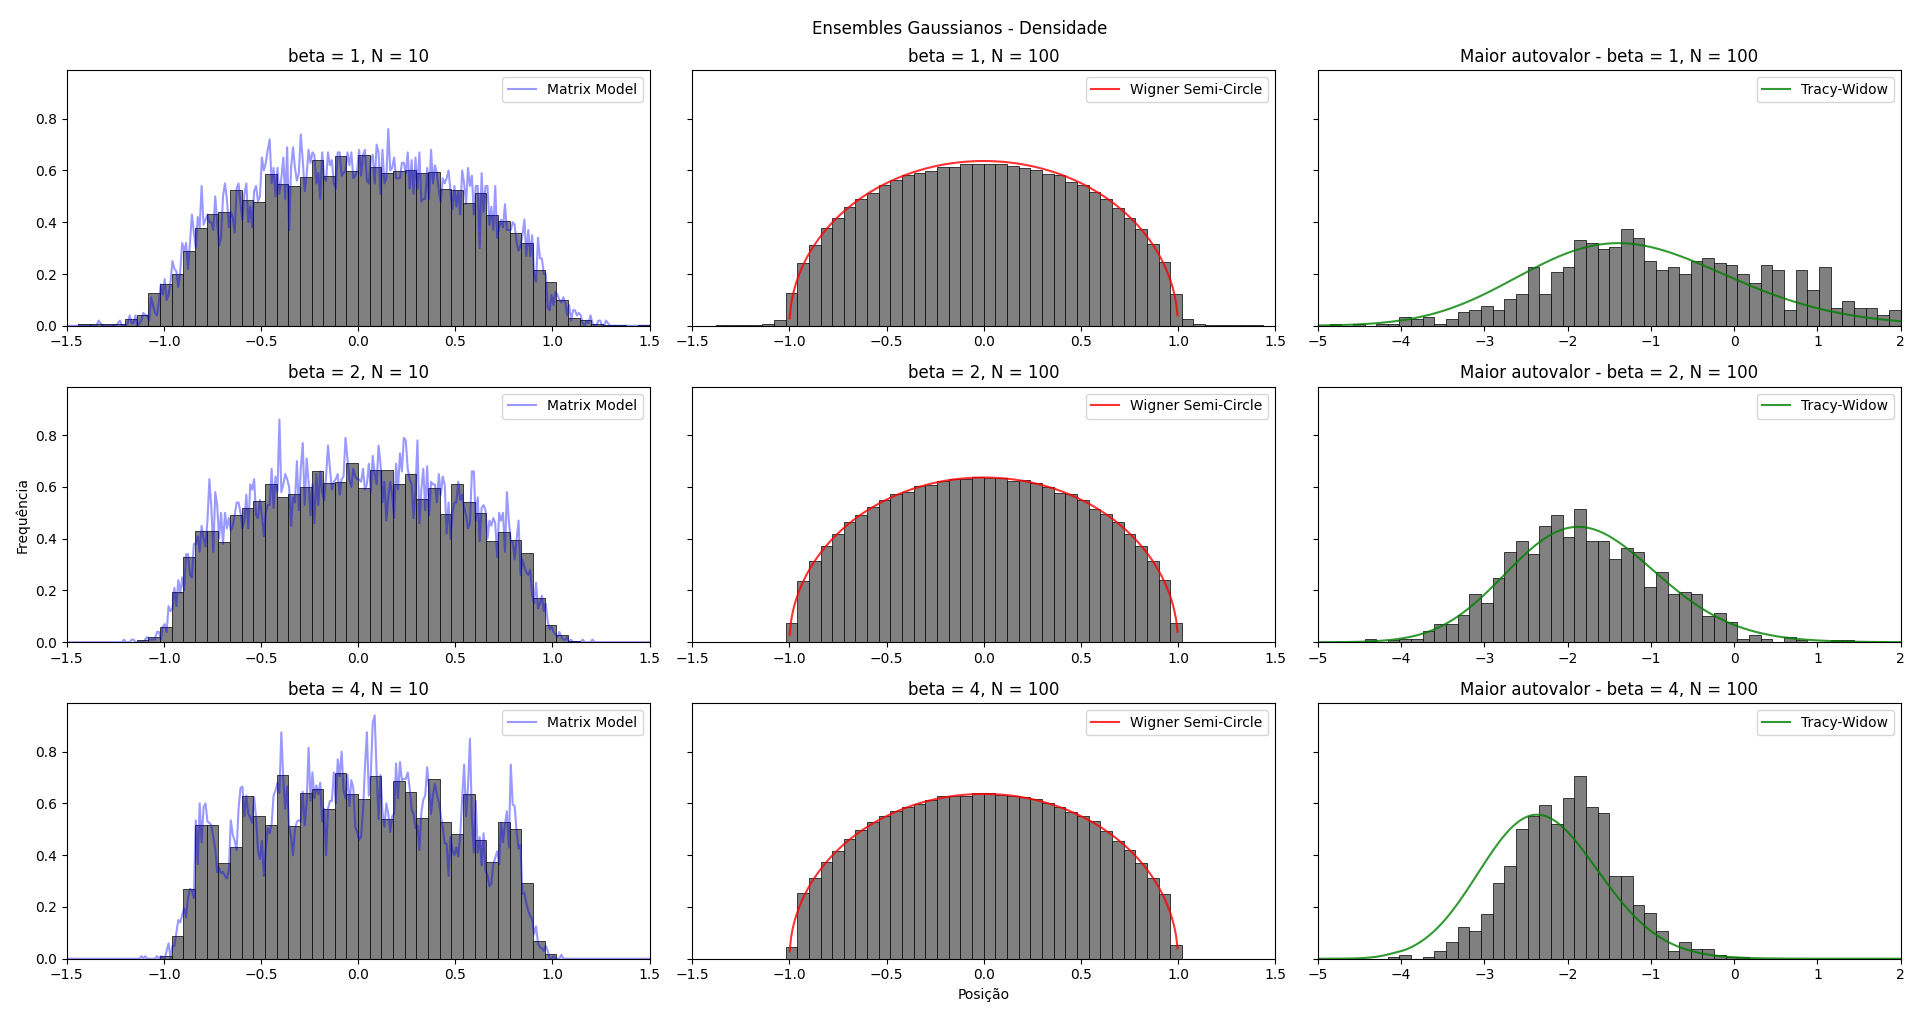
\includegraphics[width=\textwidth]{Assets/validationGaussianTracy.png}
	\caption{Medidas de equilíbrio para os ensembles gaussianos, equivalente à tomar \ref{Equation: Parametros Gaussian}. Para todos, vale a escolha de $\Delta t = 0.5$ e $nsteps = 2\cdot10^6$ passos, registrando a cada $1000$ iterações os microestados a partir da metade da simulação. Para as simulações à esquerda da figura se apresenta ainda a distribuição da amostragem de $10^6$ matrizes do tipo apropriado e a densidade resultante.}
	\label{Figura: Gaussian}
\end{figure}


% -
% C3S3 - Outros Potenciais?
% - 
%\section{Discussão}

É fácil ver para os casos \ref{Equation: Parametros Gaussian}, \ref{Equation: Parametros Monico}, \ref{Equation: Parametros Quartico} que as medidas explícita pela teoria são concordantes, como esperado, com a medida experimental obtida nas simulações. Contudo, isso é bem explorado e pode ser observado, com exceção do Mônico, em \cite{Chafa2018}. Foi discutido no Capítulo \ref{Capitulo: Intro} que os modelos gaussianos são os únicos em RMT com invariância por rotação e independência das entradas. Fica então a questão de como gerar matrizes de outros modelos se as entradas são correlacionadas. Sabemos do teorema espectral que, para as matrizes tomadas, vale a decomposição $\matriz{M} = \matriz{U} \matriz{D} \matriz{U}^{-1}$, já apresentada no Capítulo \ref{Capitulo: Intro}. Sabemos ainda que trataremos de ensembles invariantes, ou seja, a medida é a mesma para quaisquer $M, M'$ tais que $\matriz{M} = \matriz{U} \matriz{M'} \matriz{U}^{-1}$. Isso implica que podemos simular $\matriz{U}$ autovetores uniformemente do espaço correspondente. Para reconstruir uma elemento do ensemble de interesse nos resta replicar a medida de autovalores, $\matriz{D}$. Isso pode ser feito pela simulação descrita. Reconstruímos elementos dos ensembles a partir da simulação de sua medida com gases de Coulomb.
